\begin{figure}[ht]
    \centering
    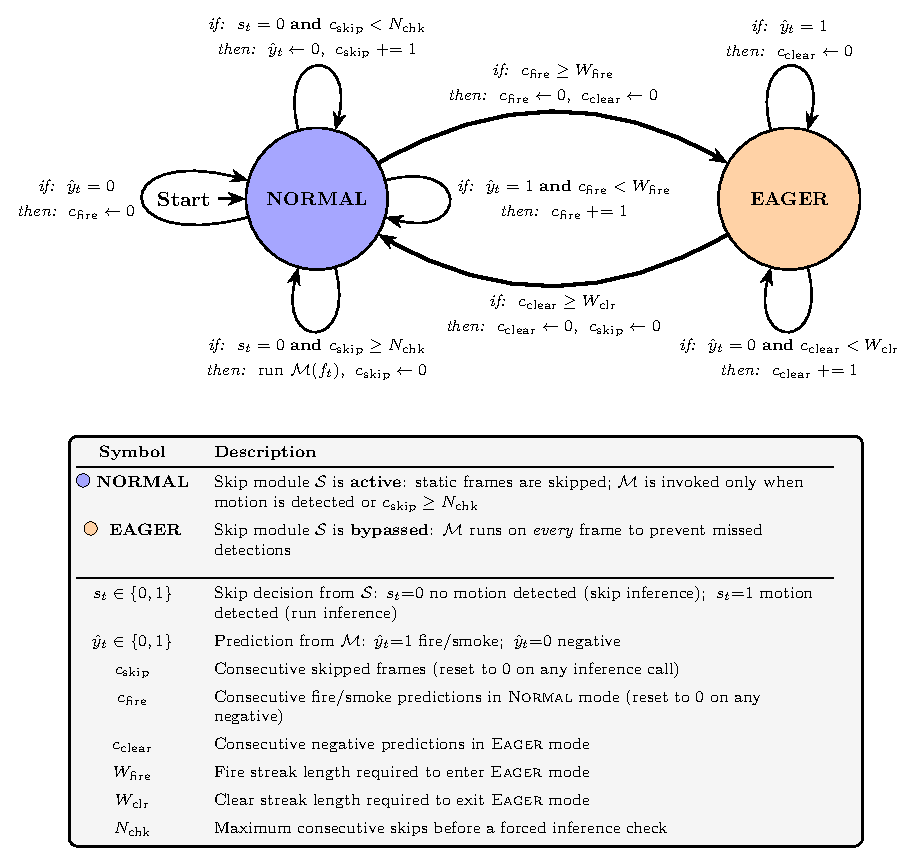
\includegraphics[width=0.8\linewidth,keepaspectratio]{./3.fig/eager/eager_mode.pdf}
    \caption{%
        State machine of the eager mode extension to the \textsc{AccMotionDet}-based
        skip module. Each transition is annotated with an \textit{if} condition
        and a \textit{then} action specifying variable updates.
        In \textsc{Normal} mode, $\mathcal{S}$ gates inference: frames with no
        detected motion are skipped and $c_{\mathrm{skip}}$ is incremented until
        $c_{\mathrm{skip}} \geq N_{\mathrm{chk}}$, at which point a forced
        inference check is issued and $c_{\mathrm{skip}}$ is reset.
        When $\mathcal{M}$ produces $W_{\mathrm{fire}}$ consecutive fire or smoke
        predictions ($c_{\mathrm{fire}} \geq W_{\mathrm{fire}}$), the system
        transitions to \textsc{Eager} mode, where $\mathcal{S}$ is bypassed and
        every frame is forwarded to $\mathcal{M}$ to prevent missed detections
        during slow-developing or settling smoke events.
        The system returns to \textsc{Normal} mode only after $W_{\mathrm{clr}}$
        consecutive negative predictions confirm that the scene is safe.
    }\label{fig:eager_mode}
\end{figure}